\chapter{Architettura di Sistema}\label{cap:Architettura}

\begin{minipage}{12cm}\textit{
		In questo capitolo verranno affrontati gli aspetti progettuali e i problemi realizzativi per poter campionare l'esperimento e trasferire i dati campionati a un dispositivo esterno collegato alla scheda principale.
	}
\end{minipage}

\vspace*{1cm}

\section{Architettura ad alto livello}\label{sec:architettura}
Il progetto finale ha come obiettivo la realizzazione di un architettura di controllo per le bobine poloidali presenti nei reattori Tokamak.

\begin{figure}[H] \label{fig:archietturaControllo}
	\centering
	\caption[Schema finale dell'archiettettura di controllo]{Architettura di controllo}
	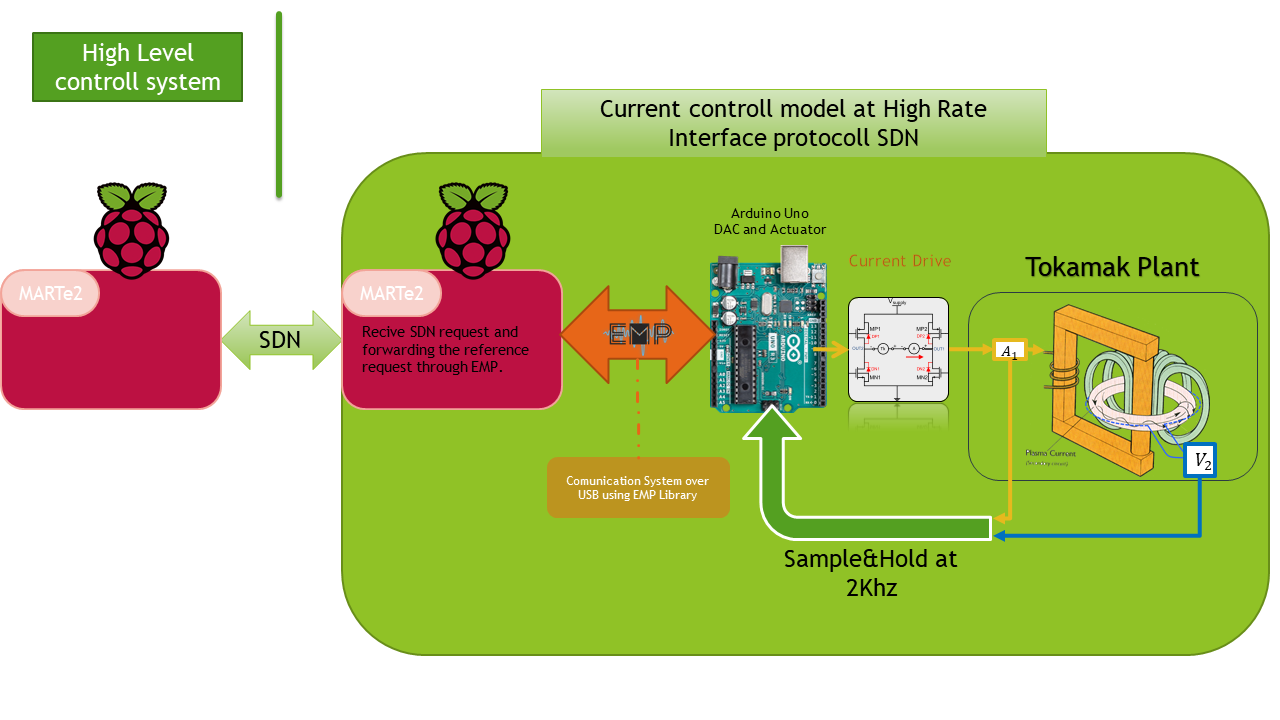
\includegraphics[width=1\textwidth]{Architettura/SystemArchitetture.png}
\end{figure}

\noindent
Lo schema proposto realizza l'obiettivo per una singola bobina, il progetto finale prevederà la ripetizione in serie del medesimo schema per il numero di bobine necessarie.\\
Dallo schema risulta evidente che tutti i componenti visti nel capitolo "\nameref{cap:Hardware}" si relazionano con lo stesso \microControllore: l'\ArduinoUno.\vspace{-4mm}
\begin{figure}[H]
	\centering
	\caption[Scheda Arduino Uno]{Scheda Arduino Uno}
	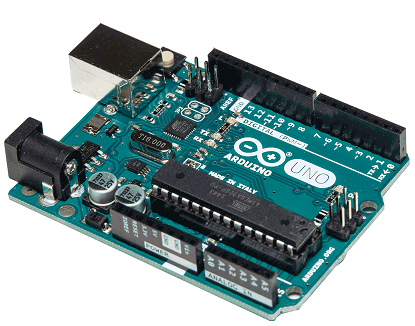
\includegraphics[width=0.45\textwidth]{Architettura/ArduinoUno.png}
\end{figure}\vspace{-6mm}

\noindent
Per riportare i dati fuori e ricevere il riferimento da inseguire nella $V_2$, è stata realizzata dal sottoscritto la libreria \cite*{EMP}.\\
La libreria è scritta in C++ ed usa fortemente il concetto di classi template per permettere ai compilatori di ottimizzarla al massimo durante la compilazione della libreria. Tra le necessità a cui deve venire in contro la libreria troviamo prima fra tutte la necessità di poter essere compilata Cross-Platform, il ché ha portato a sviluppare il codice usando il minor numero possibile di librerie esterne, le quali solo davvero universali e alla base di qualunque Toolchain, e definire il resto al suo interno.\\
Il suo compito specifico, in questo progetto, è di mettere in comunicazione l'\ArduinoUno con un nodo \MARTe installato su di una \Rasp.\\
Quest'ultimo nodo ha il compito di mettere in rete il feedback dell'esperimento, e comunicare all'\ArduinoUno eventuali cambio di riferimento. Questo ultimo tratto è realizzato mediante il protocollo \textbf{SDN}, che viaggia sopra Ethernet e dà garanzie Real-time.\\
Nella sua forma finale, il progetto prevede la riproduzione in serie di questo schema di controllo per arrivare a controllare tutte le bobine poloidali presenti in un tokamak.

\newpage

\section*{EMP - Libreria di Comunicazione Seriale\\ (Embedded Message Pack)}\label{sec:EMP}
\addcontentsline{toc}{section}{\protect\numberline{\thesection} EMP - Libreria di Comunicazione Seriale}
\vspace{-5mm}
\begin{figure}[H]
	\centering
	
\includegraphics[width=0.8\textwidth]{EMP/EMP-Logo-Background.png}
\end{figure}\vspace{-10mm}
\paragraph{\cite*{EMP}} nasce con l’obiettivo di standardizzare un protocollo di comunicazione tra 2 dispositivi, richiedendo all'utilizzatore della libreria di definire la struttura dei pacchetti che vuole trasferire, e demandando ricezione, trasmissione e verifica di integrità alla libreria.\\
La realizzazione della libreria è stata guidata dall'obiettivo di avere un'alta efficienza computazionale e un footprint di memoria uso minimo e allocabile in fase di compilazione, eliminando la necessità di memoria dinamica.\\
Lo scenario di utilizzo principale è il mettere in comunicazione 2 sistemi agli estremi di un link (rete Peer2Peer ) e non ha nessuna pretesa di networking, possibili link di comunicazione adatti sono: USB, UART, Bluetooth, moduli XBEE, etc...\\
In oltre la libreria è in grado di aggiungere un layer software per la verifica di integrità, testata attraverso un codice \cite*{CRC8} aggiunto alla fine della comunicazione dal trasmettitore, e usato dal ricevitore per decidere se scartare o tenere il pacchetto ricevuto.\\
Il protocollo usato per codificare la comunicazione è \cite*{COBS}, il quale permette di raggiungere gli obiettivi di efficienza e rapidità computazionale e porta con se la possibilità di poter supportare altre features interessanti:
\begin{spacing}{1.25}
	\begin{description}
		\item[Multiple-Package] Il protocollo di comunicazione usato (\cite{COBS}) permette di far gestire ad EMP il trasporto, attraverso lo stesso mezzo, di \textit{\textbf{pacchetti di tipologia e dimensione diversa}} senza inviare più byte di quelli strettamente necessario.\\
		\phantom{.}\hfill$\Rightarrow$ \textbf{Alta Efficienza}
		\item[Zero Tempo di negoziazione] Il protocollo di comunicazione usato (\cite{COBS}), rende EMP adatto ad un uso ‘Streaming’, questo perché non è necessario alcuna fase di sincronizzazione iniziale o durante la trasmissione in caso di perdita di dati, in aggiunta a ciò, EMP è in grado di scartare pacchetti errati in maniera trasparente all’utilizzatore. Tutto questo grazie al protocollo che \textbf{Auto-delimita i singoli pacchetti}.\\
		\phantom{.}\hfill$\Rightarrow$ \textbf{Trasparenza Totale}

	\end{description}
\end{spacing}
\noindent
Entrambe queste features aggiuntive sono presenti all'interno di \cite*{EMP} e attraverso l'uso della libreria sfruttarle è davvero semplice, le uniche responsabilità a carico degli utilizzatori è la definizione dei pacchetti che sarà possibile scambiare in fase di compilazione del codice e il riempimento corretto dei pacchetti.\\
\phantom{.}\hfill$\Rightarrow$ \textbf{Semplicità d'uso}\\
Vedremo ora di approfondire come avviene la codifica del pacchetto, così da capire come sia possibile realizzare queste funzionalità accessorie, per poi spostarci ad analizzare la struttura del codice della libreria e una rapida descrizione della direzione di sviluppo che si è presa. 

\newpage

\subsection*{Consistent Overhead Byte Stuffing (COBS)}
\addcontentsline{toc}{section}{\protect\numberline{\thesection} Protocollo - COBS}
Il protocollo di comunicazione che permette l’invio di \textbf{pacchetti diversi} e \textbf{senza fasi di negoziazione} alla base della libreria è \textbf{COBS}(\cite{COBS}).\\
Si tratta di un algoritmo per la codifica di byte, progettato per essere al tempo stesso efficiente e non ambiguo, che permette la definizione di \textit{data-pack frame} \textbf{Auto-delimiti} .

\begin{figure}[H]
	\centering
	\caption[Esempio di COBS]{Esempio di COBS}
	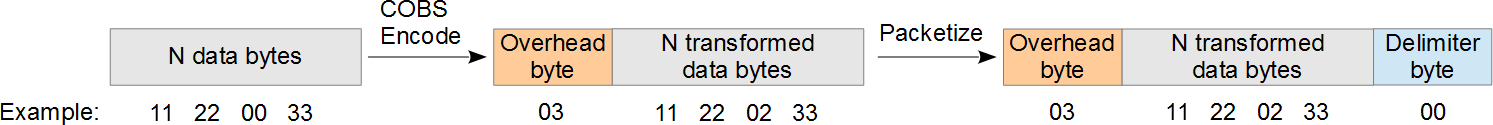
\includegraphics[width=1\textwidth]{EMP/Cobs_encoding_with_example.png}
\end{figure}

\subsection{Metodo di codifica}
L'algoritmo di COBS trasforma una stringa arbitraria di byte, ciascuno dei quali ha un Range di valori da \textbf{[0:255]} in una nuova stringa di byte dove però ogni byte va da \textbf{[{\color{red}1}:255]}. La dimensione della nuova stringa è sempre pari alla dimensione della precedente +1.\\
L'obiettivo di questo metodo di codifica è di eliminare tutti i possibili byte \zeroByte dal pacchetto in maniera reversibile.\\
Questo processo rende il carattere \textbf{\zeroByte (byte zero)} ottimo candidato per essere usato come terminatore di stringa (di byte) durante l'invio, rendendo un pacchetto COBS-Encoded mai ambiguo e sempre \textbf{Auto-delimitato}.\\
L'algoritmo di codifica consiste nel:\vspace{-5mm}
\begin{enumerate} [itemsep=-3mm]
	\item Inserire un byte \zeroByte all'inizio del pacchetto
	\item Individuare tutti gli altri byte \zeroByte
	\item Inserire un byte \zeroByte alla fine del pacchetto
	\item Sostituire tutti gli \zeroByte con la distanza dal successivo \zeroByte nella stringa, ignorando l'ultimo
\end{enumerate}\vspace{-8mm}

\begin{figure}[H]
	\centering
	\caption[Esempio di COBS con distanza]{Esempio di COBS con distanza}
	\vspace{1mm}
	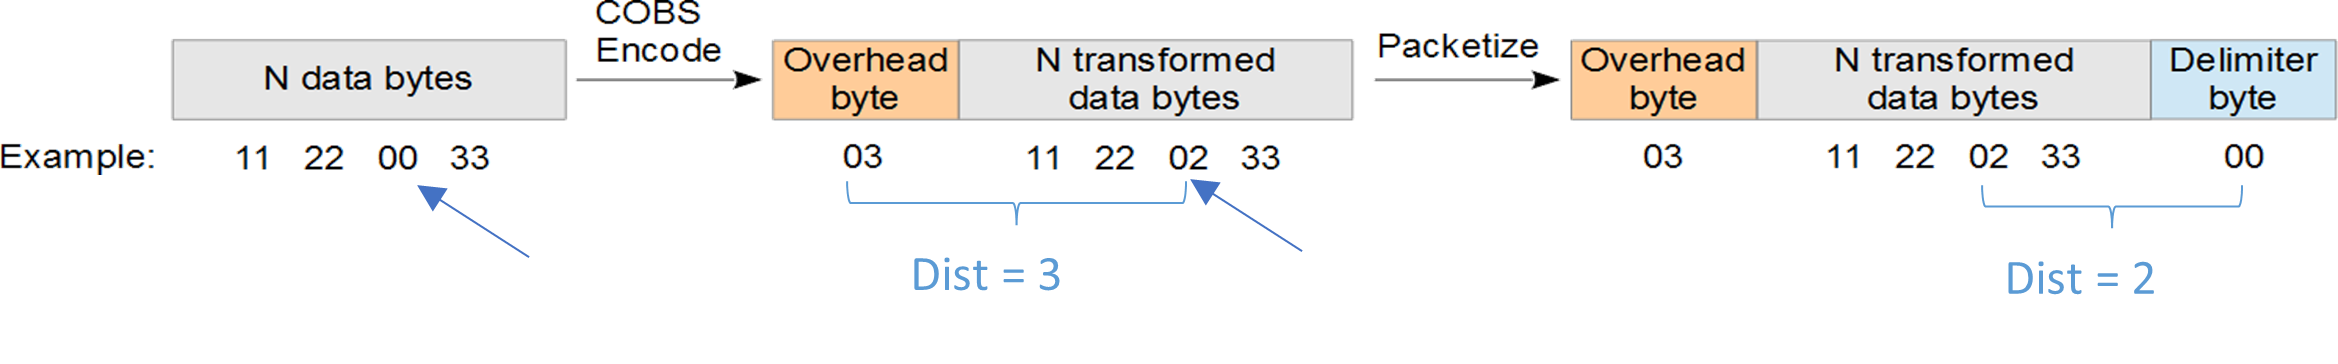
\includegraphics[width=1\textwidth]{EMP/Cobs_encoding_with_example-dist.png}
\end{figure}
\noindent
Il protocollo COBS implementato per la realizzazione di questa libreria ha il limite di non poter codificare blocchi di byte che hanno una distanza tra 2 \zeroByte superiore a 255 byte, questo limite è potenzialmente rimovibile usando un algoritmo più sofisticato, ma renderebbe il codice inutilmente più complesso e pesante da gestire poiché obiettivo EMP non è trasmettere grandi byte in sequenza, per tale motivo tale features non è stata implementata.\\
Il codice della codifica è reperibile nel repository di \cite*{EMP} al path:\\ \verb*|EMP/02_SRC/EMPlibs/src/MPcore/cobs-c/|.

\subsection{Caratteristiche chiave}
Prima caratteristica vincente della libreria è il suo alto grado di adattabilità, essa infatti per poter funzionare richiede solo \textbf{2 informazioni critiche} (e altre di contorno per l'allocazione opportuna dei buffer), esse sono i tipi dei pacchetti in \textbf{ Input} (\textit{pIn}) e in \textbf{Output} (\textit{pOut}) ovvero sia delle strutture in C, con i dati organizzati in base al messaggio da trasferire (\nameref{lst:EMPpackDef}).\\
In secondo luogo, la codifica \cite*{COBS}, che abbiamo appena visto permette di avere pacchetti \textbf{Auto-delimitati}, ciò permette quindi di scambiare pacchetti diversi tra loro (sia per tipologia che per lunghezza) lungo \textbf{lo stesso} \textit{Stream} di dati.\\
L'unica condizione neccessaria è che il destinatario sia capace di determinare la tipologia di contenuto trasportato nel pacchetto semplicemente leggendolo.\\
Questo può essere facilmente risolto in più modi:
\begin{spacing}{1.5}
	\begin{description}
		\item[Lunghezza Univoca] Ogni possibile pacchetto ha una lunghezza diversa da tutti gli altri\\
		      	\phantom{.}\hfill$\Rightarrow$ La lunghezza implica il contenuto
		\item[Aggiunta di un campo Tipologia] Aggiungendo al’inizio della trasmissione un \textit{type byte}\\
		      	\phantom{.}\hfill$\Rightarrow$ I tipi vengono Preconcordati/Standardizzati
	\end{description}
\end{spacing}
\noindent
Il metodo più universale è sicuramente l'aggiunta di un campo fisso per il tipo, di cui un esempio è visibile nell'appendice al listato \ref{lst:EMPmultiplePack} (\nameref{lst:EMPmultiplePack}).\\
In ogni caso, la codifica \cite*{COBS} aggiunge 2 byte extra al pacchetto che si vuole inviare, e tanto per la codifica quanto per la decodifica in ricezione, il \textbf{costo} è sempre pari a \textbf{O(n)}.\\
L’aver usato \cite*{COBS} come sistema di codifica per la trasmissione, garantisce che la decodifica debba avvenire solo per byte compresi tra 2 zeri, e se questa decodifica presenta un errore, toglie ogni ambiguità sul da farsi. Il Pacchetto può essere solo scartato e si torna in attesa del successivo 0 mentre si memorizzano i byte ricevuti nel mentre.\vspace{-8mm}
\begin{multicols}{2}
	\begin{center}
		{\large \color{dkgreen}Vantaggi:}
	\end{center}
	\begin{spacing}{1.25}
		\begin{enumerate}[itemsep=-1mm]
			\item Pacchetti {\color{cadmiumgreen}\textbf{Self-Delimited}}
			\item Canale {\color{cadmiumgreen}\textbf{Multi-Packet ready}}
			\item Protocollo {\color{cadmiumgreen}\textbf{Senza Negoziazioni}}
			\item Responsabilità minime per l'utilizzatore
			\item Prerequisiti implementativi minimale (mezzo di comunicazione \textit{peer2peer} asincrono)
		\end{enumerate}
	\end{spacing}
	\vfill
	\columnbreak
	\begin{center}
		{\large \color{red} Svantaggi:}
	\end{center}
	\begin{spacing}{1.25}
		\begin{enumerate}[itemsep=-1mm]
			\item Aggiunge 2 byte fissi
			\item Richiede O(n) elaborazione sia in codifica che decodifica
		\end{enumerate}
	\end{spacing}
	\vspace*{\fill}
\end{multicols}

\subsection{Integrità dei pacchetti}\vspace{-2mm}
Per aumentare ulteriormente i campi d’uso e garantire un layer minimale di \textbf{integrità} sui pacchetti in transito, la libreria è in grado di include in maniera trasparente anche un un check di errore calcolato usando \cite{CRC8}, aggiunto in trasmissione e rimosso in ricezione. L'aggiunta e la verifica del CRC8 viene fatta sul pacchetto non ancora \textit{COBS-Encodato}, ciò garantisce la possibilità di inviare il pacchetto a prescindere da quale sia il risultato del CRC8, e viene quindi verificato dopo aver de-\textit{COBS-Encodato} il pacchetto in ricezione.\\
Questa features può essere agevolmente attiva o disattivata in fase di compilazione, ma necessita di essere attiva o disattiva contemporaneamente su entrambi i lati del link.\\
Se attiva essa è in grado di far capire se il pacchetto ha subito degli errori (ovviamente nei limiti del CRC8) e in tal caso scarta il pacchetto ricevuto in maniera totalmente trasparente all'utilizzatore che non ne vien notificato.\\

\newpage
\subsection{Struttura del codice}
Lo sviluppo del codice è qui riassunto nel \textbf{Class Diagram} fatto in UML, del codice:
\begin{figure}[H]
	\centering
	\caption[Class Diagram UML di EMP]{Class Diagram UML}
	\includegraphics[width=1\textwidth]{EMP/EMP-Hierarchy.png}
\end{figure}
\noindent
Senza entrare eccessivamente nel dettaglio di \citefield{EMP}{title}, essendo tutto reperibile nella versione più aggiornata all'interno del repository di \cite*{EMP}, osserviamo che il codice è diviso in 2 macro blocchi (\textbf{MPCore}, \textbf{MP}) più una classe di supporto per il buffer circolare.\\
Questa organizzazione del codice è stata pensata per far compilare su tutte le piattaforme di interesse lo stesso \textit{codice attivo} (codifica e decodifica dei pacchetti+accumulo), e demandare le particolarizzazioni dovute alle varie piattaforme o al mezzo di comunicazione usato nel caso specifico a delle classi figlie.\\
\begin{spacing}{1.25}
	\begin{description}
		\item[MPCore] Il \textit{Codice attivo} è presente all'interno del package \textbf{MPCore}. Tutto il codice contenuto in questo package è scritto in C++11 e per essere compilato necessita di un set minimale di librerie standard, sicuramente presenti in ogni piattaforma di sviluppo.
		\item[EMP] Il package più generico comprende le classi figlie che concretizzano le operazioni di invio e ricezione, facendo poi elaborare i byte al codice che ereditano dalla classe \textbf{MP}.\\
		      Le classi sono scritte e pensate per funzionare su una piattaforma specifica, e su essa essere ottimizzate.\\
		      Se la piattaforma lo concede come nel caso di Linux, è quindi possibili fattorizzare ulteriormente delle funzionalità comuni e scrivere così, via via, sempre meno codice sicuri che quello in comune, se funziona su una classe, deve funzionare anche per l'altra.
		\item[Buffer Circolare] La classe \textit{CircularBuffer} è una classe di supporto che implementa un buffer circolare con logica "\textit{One Slot Open}"(\cite{CircularBuffer}) attraverso una classe template.\\
		      Il motivo di questa scelta, molto forte e vincolante, essendo principalmente lei la causa per cui tutte le altre sono anch'esse template, è dovuta alla possibilità di istanziare in fase di compilazione, tutta la memoria richiesta per il funzionamento del programma.\\
		      Una simile necessità nasce dal dover compilare la classe anche su schede embedded, le quali, notoriamente, non hanno a disposizione un heap in ram spazioso per la memoria dinamica, e beneficiano nelle prestazioni se in fase di compilazione gli indirizzi di memoria sono fissi.
	\end{description}
\end{spacing}
\vspace{0mm}
\subsection{Logica di Comunicazione}
\vspace{-5mm}
La libreria è pensata per automatizzare la trasmissione e la ricezione di 2 tipologie di pacchetti \textit{Pre-concordati} tra 2 realizzazioni di \textbf{MP}, ovviamente non necessariamente sullo stesso dispositivo.\\
Come riportato in Appendice B (\ref{EMPCode}), la definizione dei pacchetti è pensata per essere molto comoda e naturale. In oltre usando un campo per distinguere il tipo di pacchetto e una \verb|union| per unire in un unica area di memoria pacchetti differenti, è anche possibile gestire la comunicazione di pacchetti multipli tra i 2 lati della comunicazione, basterà invertire l'ordine dei tipi tra le 2 classi ai 2 estremi della comunicazione.\\
Il riempimento corretto dei dati nel pacchetto, il calcolo della \textit{size} reale di invio (per evitare sprechi) e il riconoscimento in ricezione del pacchetto trasmesso, è tutto a carico dell'utilizzatore della libreria, essa garantisce la corretta ricetrasmissione e di svegliare un ascoltatore al ricevimento di un pacchetto, qualunque sia la lunghezza ricevuta purché sia codificato correttamente, e in caso di CRC8, non presenti errori .


\newpage
\subsection{Code Flow}\label{sub:codeFlow}
Vediamo ora come la libreria si frappone tra 2 device che vogliono comunicare mediante questo sequence diagram:
\begin{figure}[H]
	\centering
	\caption[Sequence Diagram UML di EMP]{Sequence Diagram UML}
	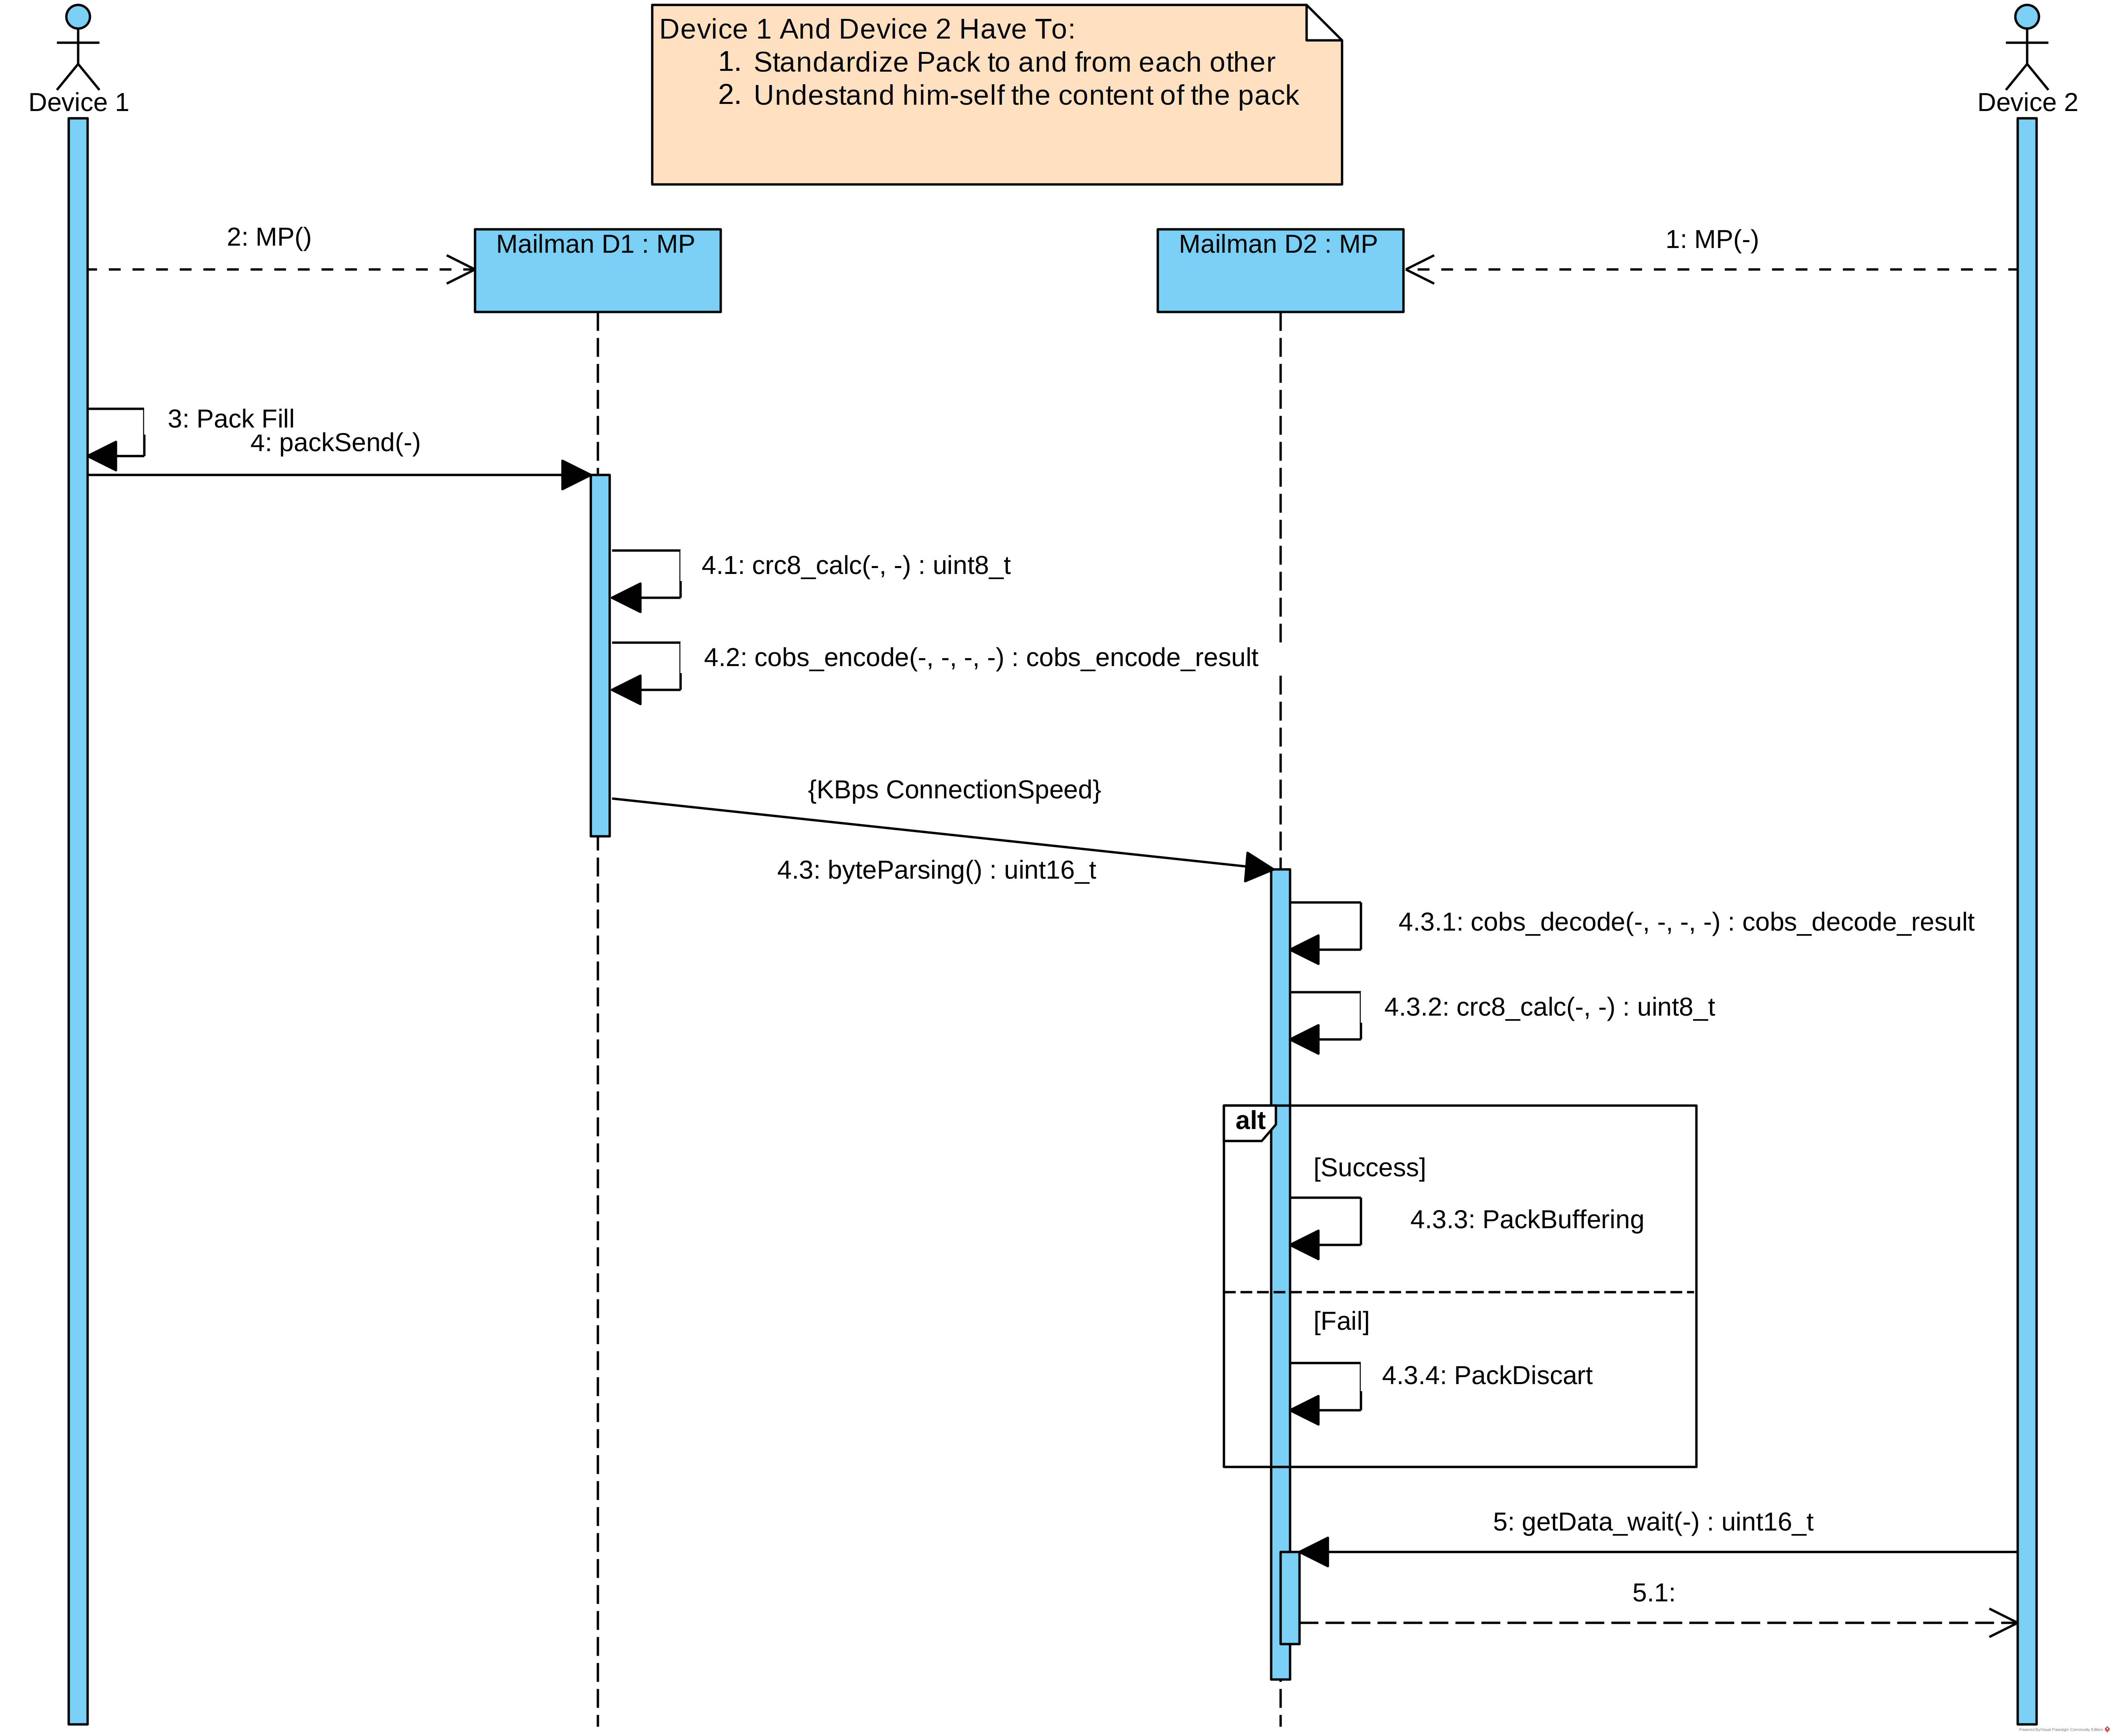
\includegraphics[width=1\textwidth]{EMP/Message Pack Sending Flow.png}
\end{figure}
\noindent
In questo esempio generico i 2 device non sono definiti, ovviamente nessuno dei 2 può istanziare concretamente una classe \textbf{MP}(essendo una classe virtuale), ma come detto prima, tutti i \textit{Codici attivi} sono racchiusi lì dentro.\\
Come si può osservare, eccetto il riempire i dati, inviarli e attendere che arrivi qualcosa, per gli attori il lavoro finisce subito, internamente alla libreria, invece, a parti invertite, abbiamo il calcolo del CRC8 (\cite{CRC8}) e la codifica usando COBS (\cite{COBS}), e l'omologo dall'altro lato, dopo aver ricevuto i byte, procede alla de-codifica e check per l'integrità.\\

\subsection{Test di Codifica/Decodifica su ogni Device}
La serie di passi descritta nel \nameref{sub:codeFlow} è stato testato su i vari dispositivi per cui la libreria è stata sviluppata usando il seguente schema:
\begin{figure}[H]
	\centering
	\caption[EMP Benchmark Testing Flow]{Testing Flow}
	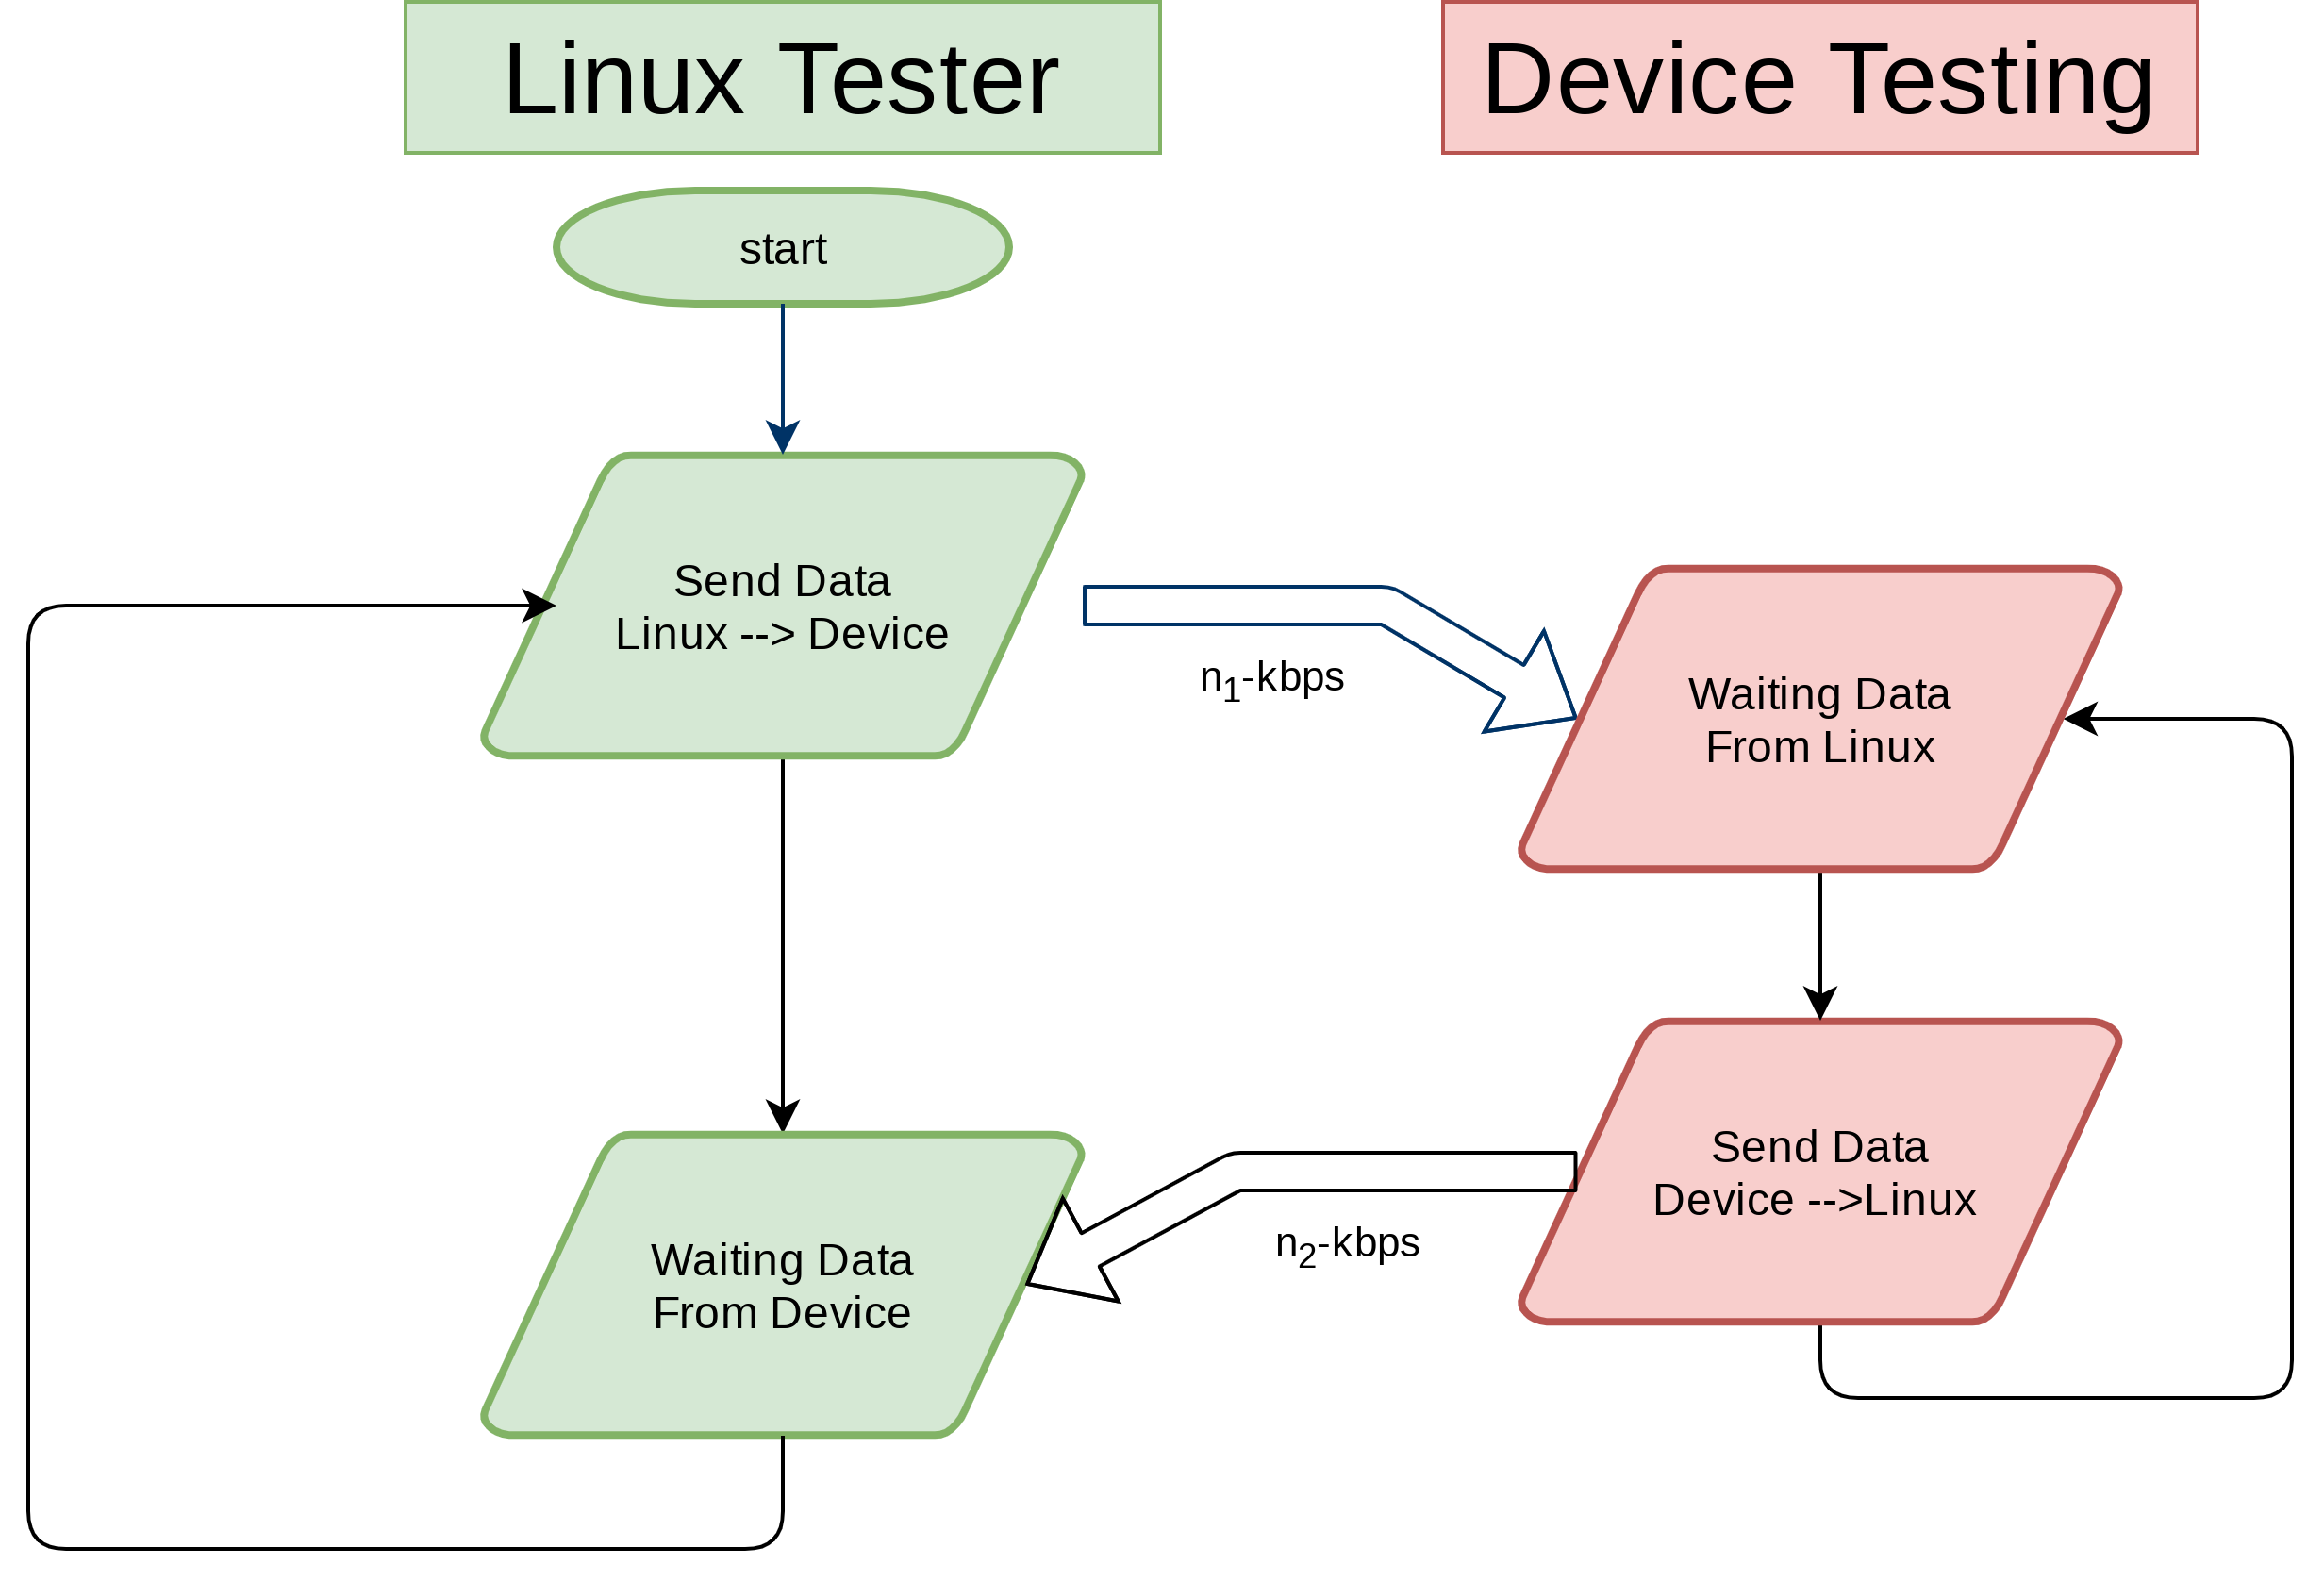
\includegraphics[width=0.8\textwidth]{EMP/TestFlow.png}
\end{figure}

\noindent
I test vengono avviati da \textbf{Linux} e puntano a testare la perdita la correttezza della trasmissione usando \citefield{EMP}{title}, e il funzionamento di Encoding e Decoding delle classi sulle entrambe le architetture.\\
Ad ora, sulle 3 Piattaforme di sviluppo (Linux, Arduino, STM32) i test sono stati un pieno successo.

\newpage
\section{Online Sampling}
Come descritto in figura \ref{fig:archietturaControllo}, il sistema controlla internamente la corrente, ma comunica con il mondo fuori l'attuale stato della bobina.\\
Per comunicare i Sample (e ricevere le Reference) è stata usata \citefield{EMP}{title}(Sezione \ref{sec:EMP}).\\
Come visto nella sezione '\nameref{sub:parametriMisurati}', il circuito di misura è quello riportato in figura \ref{fig:circuitoDiMisura}.\\
E, come per il \nameref{CurrentSense}, in realtà anche il voltmetro $V_2$ possiede un offset a $\frac{V_{cc}}{2}$, aggiunto per poter misurare tanto le correnti positive, quanto quelle negative.\vspace{-2mm}
\begin{figure}[H]
	\centering
	\caption[Circuito equivalente del Plasma con l'offset delle Misure]{Circuito reale con Misure}\vspace{2mm}
	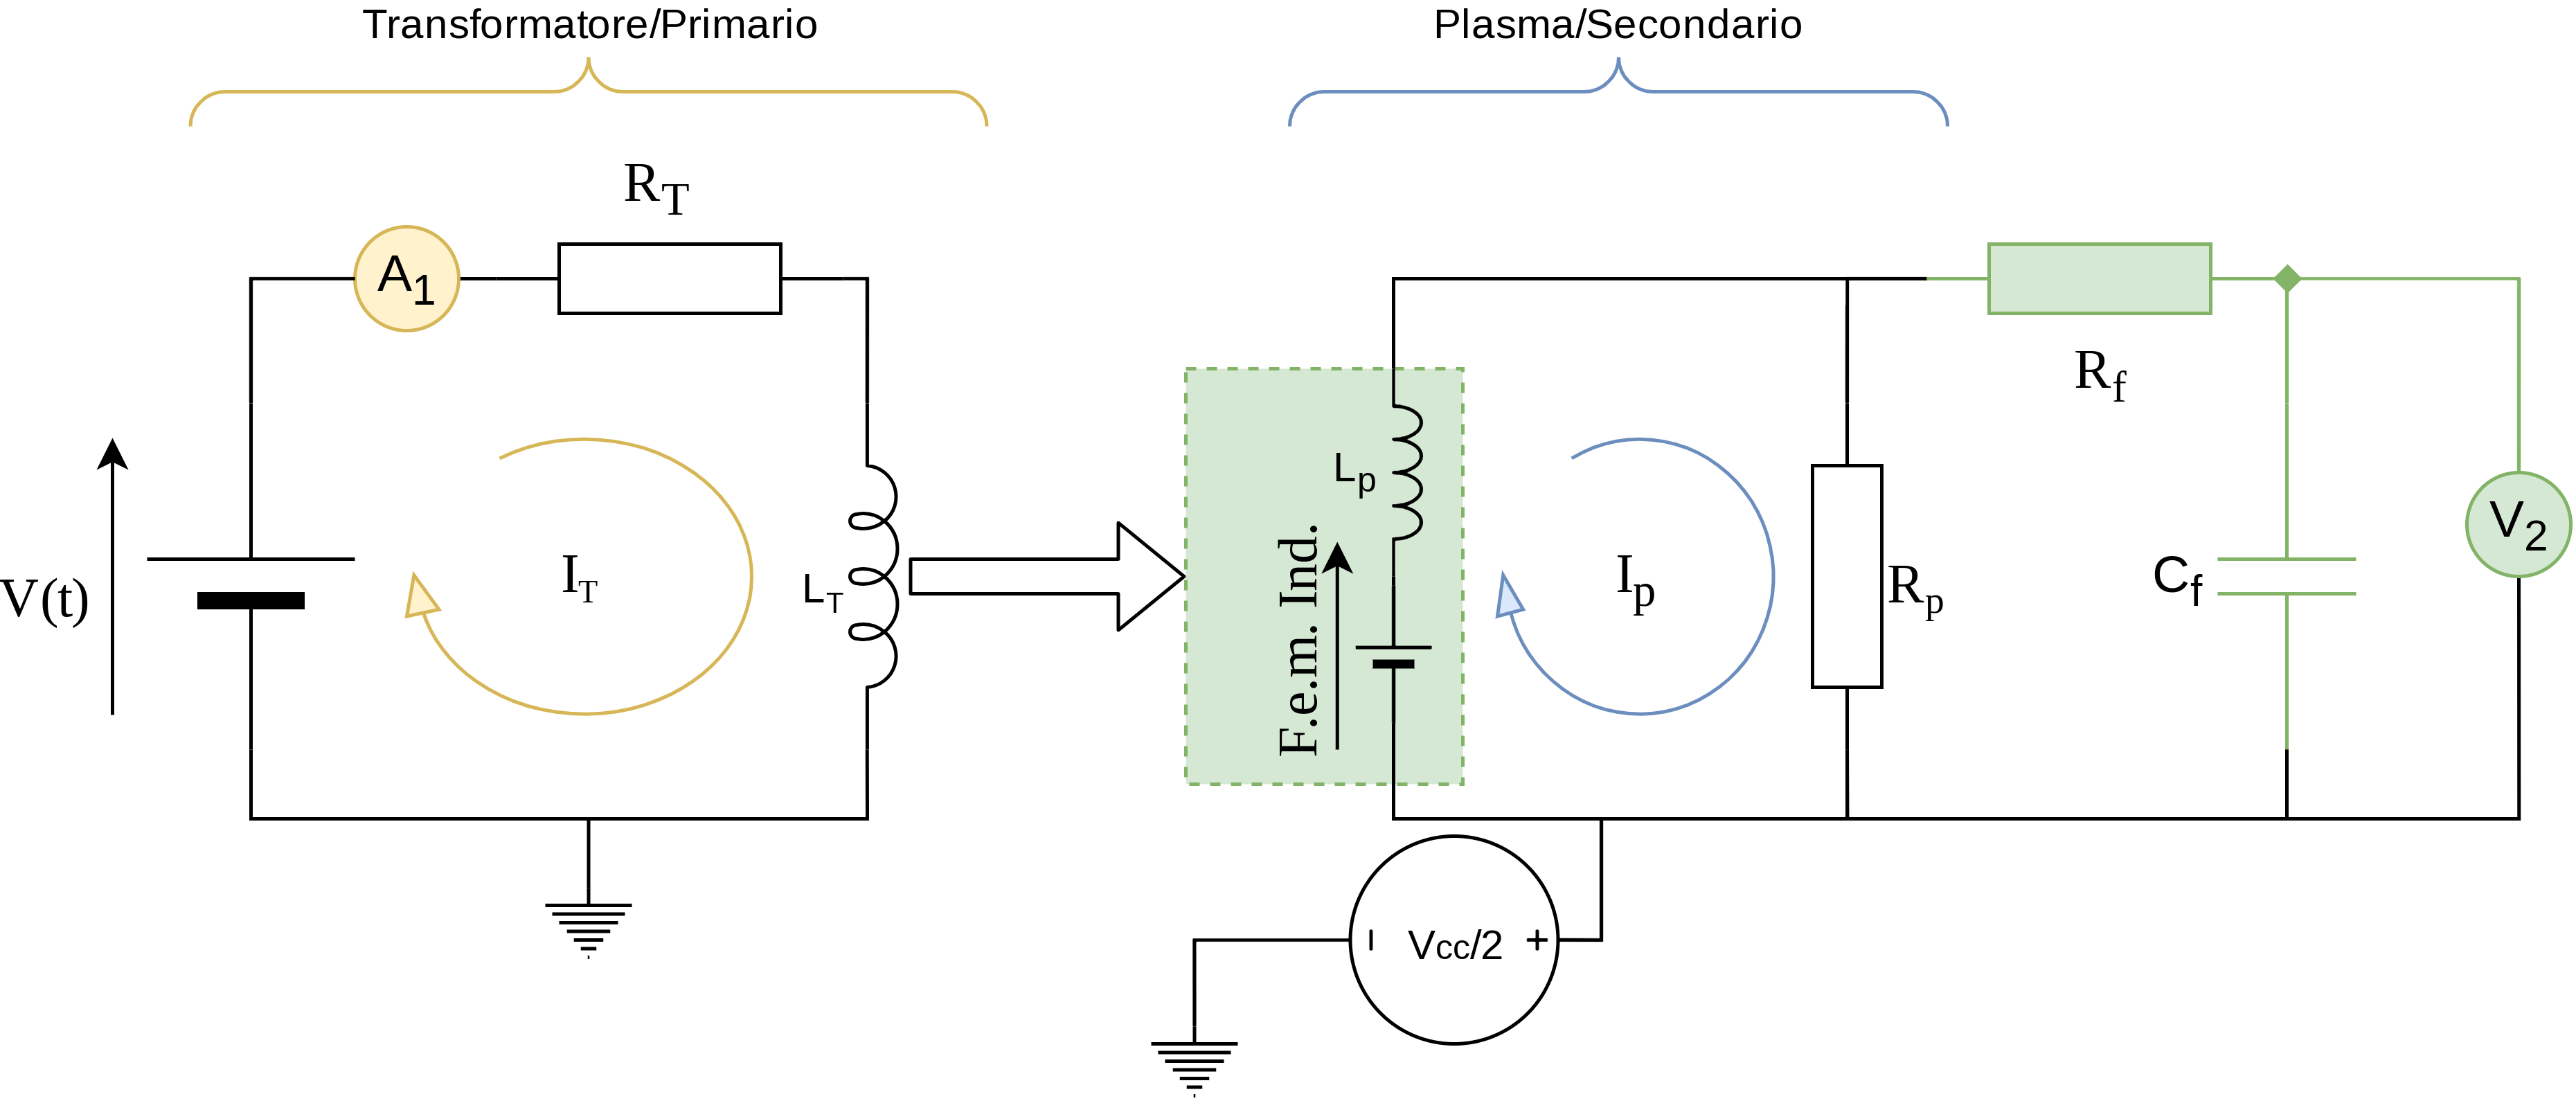
\includegraphics[width=1\textwidth]{Trasformatore/PlasmaCircuit-MisureCircuitOffset.png}
\end{figure}
\noindent
Controllo e misure avvengo alla massima frequenza che l'Arduino riesce effettivamente a gestire, ovvero 0.5ms (2Khz), nei quali campiona lo stato del sistema, attua il nuovo valore del PWM  calcolato per il controllo $V(t)$, e invia i dati attraverso \cite*{EMP}.

\newpage
\subsection{Interconnessione \microControllore $\Leftrightarrow$ Companion}
Per raggiungere gli obiettivi descritti nella sezione dell'\nameref{sec:architettura}, i seguenti pacchetti multipli sono stati concordati tra le 2 parti:
\begin{lstlisting}[style=cppStyle,caption={Pacchetti Companion $\Rightarrow$ \microControllore   },label=lst:Companion2ArdPack]
// #######################################################
// ########        Companion to Arduino           ########
// #######################################################
struct newRef {
	int16_t newRef;
} __attribute__((packed));

struct setUpPackAsk {
	int8_t padding;
} __attribute__((packed));

enum LinuxSendType : uint8_t { newRefType, askType };

struct _packLinux2Ard {
	LinuxSendType type;
	union {
		struct newRef ref;
		struct setUpPackAsk ask;
	};
} __attribute__((packed));
typedef struct _packLinux2Ard packLinux2Ard;
\end{lstlisting}

\begin{lstlisting}[style=cppStyle,caption={Pacchetti \microControllore $\Rightarrow$ Companion },label=lst:Ard2CompanionPack] 
// #######################################################
// ########        Arduino to Companion           ########
// #######################################################
struct sample {
	int16_t pwm;
	int16_t V2_read;
	int16_t Isense_read;
	int16_t err;
} __attribute__((packed));

struct setUpPack {
	int16_t V2_mean;     // Adc read
	int16_t Isense_mean; // Adc read
	int16_t dt;          // Time in us (10^-6)
} __attribute__((packed));
enum ardSendType : uint8_t { sampleType, setUpPackType };

struct _packArd2Linux {
	ardSendType type;
	union {
		struct sample read;
		struct setUpPack setUp;
	};
} __attribute__((packed));
typedef struct _packArd2Linux packArd2Linux;
\end{lstlisting}
\noindent
Essi permettono al Companion di conoscere tutto quello che sta succedendo nel \microC, con un piccolo ritardo dovuto alla trasmissione ed eventuali ritardi interni (nel caso di Linux dovuti allo scheduler).
Le informazioni riguardanti offset e parametri dell'esperimento (\verb|struct setUpPack|), sono raccolti a esperimento fermo, in particolare all'accensione della scheda nel \nameref{lst:controlSetup}.\\
Successivamente la scheda evolve per tic di 0.5ms, dove nel tempo morto resta in ascolto di eventuali pacchetti di richiesta da parte del Companion all'interno del \nameref{lst:controlLoop}.

\subsection{Storage su file delle informazioni}\label{subsec:experimentStorage}
Le informazioni ricevute dal Companion, vengono salvate all'interno di un file di testo contenente 2 tabelle, disposte una sotto l'altra.\\
La prima delle 2, tabula i dati del pacchetto \verb|struct setUpPack|, il quale risulta utile per poter interpretare i dati successivamente.
\begin{table}[H]
	\centering
	\caption[Salvataggio di 'struct setUpPack']{Salvataggio di 'struct setUpPack'}
	\begin{tabular}[t]{|c|c|c|}
		\hline
		$ V_{2_{mean}} $ & $ I_{sense_{mean}}$ & dt  \\
		\hline
		510              & 510                 & 500 \\
		\hline
	\end{tabular}
\end{table}

\noindent
La seconda invece è lo streaming dei dati \verb|raw|, ottenuti dalla scheda:
\begin{table}[H]
	\centering
	\caption[Salvataggio di 'struct sample' $\forall$ dt]{Salvataggio di 'struct sample' $\forall$ dt}
	\begin{tabular}[t]{|c|c|c|c|}
		\hline
		PWM   & $ V_{2_{read}}$ & $ I_{sense_{read}}$ & e     \\
		\hline
		0     & 509             & 510                 & 1     \\
		0     & 509             & 511                 & 1     \\
		\dots & \dots           & \dots               & \dots \\
		0     & 509             & 510                 & 59    \\
		44    & 510             & 510                 & 36    \\
		48    & 518             & 510                 & 28    \\
		53    & 514             & 510                 & 32    \\
		59    & 513             & 510                 & 33    \\
		\dots & \dots           & \dots               & \dots \\
		\hline
	\end{tabular}

\end{table}
\noindent
Essi sono salvati sotto forma di testo ascii normale, separando i campi con un \verb|'tab'| (\verb|\t|).

\newpage
\section{Post Elaborazione con Matlab}
I dati salvati su Hard Disk, come visto della sezione \nameref{subsec:experimentStorage}, vengono presi in ingresso da Matlab e convertiti dai valori del DAC ai rispettivi fisici.

\subsection{Conversioni Dati}
Per ottenere la tensione reale letta il cambio è molto semplice:
\begin{empheq}[box=\mathResult]{equation*}
	V_{read} = ADC_{Read} \cdot V_{step}= ADC_{Read} \frac{Vcc}{2^{10}-1} = ADC \cdot 4,887mV
\end{empheq}

\noindent
Partendo da questa equivalenza, per la corrente del primario usiamo l'equazione \ref{eq:Iread}, mentre la tensione sul secondario necessita solo della cancellazione dell'offset:
\begin{empheq}[box=\mathStep]{equation} \label{eq:V2Read}
	V_2 = V_{read} - V_{2_{offset}}
\end{empheq}

\subsection{Filtraggio senza distorsioni di fase} \label{subsec:filtraggio}
Essendo i dati letti affetti naturalmente da rumore, essi vengono post-filtrati per rendere i dati più puliti e mettere in evidenza le tendenze del sistema. Questo filtraggio è stato realizzato usando un \textit{Filtro digitale a senza distorsione di fase}(\cite{zeroPhaseShiftFilter}), come fa intuire il nome, la caratteristica di questo filtro è che non introduce nessun ritardo o anticipazione al segnale filtrato, permettendo di confrontarlo direttamente con i dati puri, eliminando rumori a bassa ed alta frequenza.\\
Questo filtraggio viene eseguito direttamente nell'importazione della tabella salvata con la struttura vista nella sezione \nameref{subsec:experimentStorage}, di cui il codice è in appendice \nameref{subsec:tabParsing}.